\section{Experiments}
\label{sec:experiments}

Experiments~1--3 build the instrument: the judge-variance grid, the reversal
curves, and the noise floor. Experiment~4 applies it to a published improvement
loop, and a contrast against expert human annotations
(Section~\ref{sec:exp1}) bounds what the threshold licenses.

\subsection{Experiment 1: Judge-Variance Grid}
\label{sec:exp1}
% Full-grid runs (ledger data/ledger.jsonl):
%   exp1_dense  run_id=r_20260801_da6e9c config_hash=57230b2ac56a5ffe
%   exp1_anchor run_id=r_20260801_0eeb4b config_hash=471dabd1861b8f7a
%   exp1_alpaca run_id=r_20260801_cc2370 config_hash=6455906059207bcb
% %p normalization: raw / scale-width * 100, widths likert5=4,
% likert10=9, score100=100. Raw-scale and sigma-relative values in appendix.
Experiment~1 estimates $\sigma(\env)$ on a grid of eight environments spanning
two judges, two tasks, and three scales, and reads $\mdi_{\alpha}(\env, N)$ off
the mean-of-$N$ estimator. The dense tier is \texttt{gpt-4o-mini} (full grid);
the anchor tier is \texttt{gpt-5.6}, run on two shared summarization cells
(likert5, plus score100 for the scale contrast) to test the registered
judge-upgrade hypothesis. Tasks are SummEval summarization and AlpacaEval~2.0
instruction-following, each with four close systems
($s_{07}, s_{09}, s_{11}, s_{12}$) over 100 held items (anchor cells: 50 and
40), on the direct-scoring scales likert5, likert10, and score100.
Each (system, item) cell is scored at temperature~1 ($N{=}20$ repeats dense,
$N{=}8$ anchor; $19$ and $7$ after the screening hold-out) with the budget
swept over
$N \in \{1,3,5,8,10,20\}$, with parse failures under $0.56\%$. Call counts,
spend and config hashes are in the registry (Table~\ref{tab:run-registry}).
The $N$ argument is what separates
this from prior work: a single-call statistic such as $\Delta^*_{75}$ of
\citet{usami2026darkcurrent} has one value per judge, while
$\mdi_{.05}(\env, N)$ moves with the budget (Table~\ref{tab:exp1-lookup}). One
instrument can therefore support many decision thresholds.

\paragraph{The upgraded judge is not uniformly quieter; on the fine scale
the ordering cleanly reverses.}
Judges are compared by $\sigma$, never by $\mdi$: the anchor cells use fewer
items (Appendix~\ref{app:extra}). On coarse likert5 the costlier
\texttt{gpt-5.6} points \emph{noisier}, not quieter:
$\sigma = 7.15$~\%p [6.33, 7.89] vs.\ $6.40$~\%p [5.94, 6.84] (95\% CI,
meeting only at the margin). On fine score100 the ordering \emph{reverses},
cleanly: $2.86$~\%p [2.70, 3.01] vs.\ $3.82$~\%p [3.62, 4.00],
non-overlapping. The registered hypothesis (a judge upgrade does not by
itself reduce instability) gets a scale-dependent answer: resolution is a
joint property of judge and scale, so a coarse threshold is fixed by design,
not by a more expensive judge. Whether that
holds on other tasks is left to the expanded grid.
%% source: variance_by_env.csv (exp1_dense, exp1_anchor, exp1_anchor_scales);
%% sigma in %p = raw sigma / scale-width * 100 (likert5 width 4, score100 100).
%% likert5 raw: 4o-mini 0.256 [0.238,0.273] -> 6.40%p; gpt-5.6 0.286 -> 7.15%p.
%% score100 gpt-5.6 40 items, others 100; MDI not compared across judges here.
%% run_ids: dense r_20260801_da6e9c, anchor r_20260801_0eeb4b,
%% anchor_scales r_20260802 (score100 40-item, N=8).

\begin{table}[t]
  \centering
  \caption{Experiment 1: repeat instability $\sigma(\env)$, the two-sided
    null-PI half-width $\mdi_{.05}(\env, N)$ per budget
    (Definition~\ref{def:mdi}), and the reverse read-off, the smallest $N$
    whose MDI clears a target gain [+\%p] (``un.''$=$unreachable; a dash $=$ an
    unsupported budget). \textbf{Both are at level $\alpha$; for a stated power
    multiply by the measured factor of $1.43$ (Section~\ref{sec:framework}),
    which changes 10 of these 24 answers, 4 to unreachable; a gain just past
    $\mdi$ can still reverse (Table~\ref{tab:fip-conversion}).} All in \%p; ties
    resolved at full precision. Every column holds the prompt fixed
    (Section~\ref{sec:exp3}). Pilot estimates; raw scale:
    Table~\ref{tab:raw-sigma}. The estimator's split-half term inflates
    every entry past $N{=}1$, conservatively by $10$--$40\%$ from $N{=}3$
    to $N{=}10$ ($26$--$47\%$ anchor); factors and the corrected column are
    in Table~\ref{tab:pool-inflation}.}
  \label{tab:exp1-grid}
  \label{tab:exp1-lookup}
  %% source: paper/tables/variance_by_env.csv (sigma, flip_rate),
  %% paper/tables/mdi_table.csv (mdi_null_pp, alpha=0.05); equivalently
  %% data/derived/exp1_*/mdi_table.json ("null_entries").
  %% run_ids: dense r_20260801_da6e9c, anchor r_20260801_0eeb4b,
  %% alpaca r_20260801_cc2370 (see data/ledger.jsonl).
  \label{tab:exp1-repeats}
  \footnotesize
  \begin{tabular*}{\linewidth}{@{\extracolsep{\fill}}lcccccccccc}
    \toprule
    & & \multicolumn{5}{c}{$\mdi_{.05}(\env, N)$ [\%p]}
      & \multicolumn{3}{c}{$N$ needed for a gain of} \\
    \cmidrule(lr){3-7} \cmidrule(lr){8-10}
    Environment (judge $\cdot$ task $\cdot$ scale)
      & $\sigma$ [\%p]
      & $N{=}1$ & $N{=}3$ & $N{=}5$ & $N{=}8$ & $N{=}10$
      & $+0.5$ & $+1$ & $+2$ \\
    \addlinespace[1pt]
    \midrule
    4o-mini $\cdot$ Summ $\cdot$ L5   & 6.40 & 1.75 & 1.13 & 0.93 & 0.84 & 0.78 & un. & 5   & 1 \\
    gpt-5.6 $\cdot$ Summ $\cdot$ L5   & 7.15 & 3.00 & 2.00 & 1.85 & --   & --   & un. & un. & 3 \\
    4o-mini $\cdot$ Summ $\cdot$ L10  & 4.69 & 1.28 & 0.81 & 0.69 & 0.58 & 0.58 & un. & 3   & 1 \\
    4o-mini $\cdot$ Summ $\cdot$ S100 & 3.82 & 1.07 & 0.65 & 0.54 & 0.50 & 0.46 & 8   & 3   & 1 \\
    gpt-5.6 $\cdot$ Summ $\cdot$ S100 & 2.86 & 1.23 & --   & 0.84 & --   & --   & un. & 5   & 1 \\
    4o-mini $\cdot$ Instr $\cdot$ L5  & 4.28 & 1.25 & 0.75 & 0.60 & 0.55 & 0.53 & un. & 3   & 1 \\
    4o-mini $\cdot$ Instr $\cdot$ L10 & 3.84 & 1.11 & 0.70 & 0.54 & 0.50 & 0.47 & 10  & 3   & 1 \\
    4o-mini $\cdot$ Instr $\cdot$ S100 & 2.47 & 0.65 & 0.45 & 0.38 & 0.32 & 0.30 & 3  & 1   & 1 \\
    \bottomrule
  \end{tabular*}
\end{table}

\paragraph{The lookup, forwards and backwards.}
Figure~\ref{fig:mdi-overview} plots this table. Inside the dense tier the
threshold spans $0.65$--$1.75$~\%p at $N{=}1$ (the anchor rows reach
$3.00$~\%p on fewer items and fewer repeats, so they stay out of that ratio),
and $N{=}1 \to 5$ roughly halves it in every cell, short of the
$\sigma/\sqrt{N}$ ideal because the finite estimation pool adds a term of its
own (Appendix~\ref{app:extra}).



\paragraph{What the threshold licenses, against the expert reference.}
The close four were picked for indistinguishability; a validation pass
re-scores eleven systems spanning the reference's range, so two agreement
figures coexist: rank concordance $0.33$ on the close four, $0.855$ over
all $55$ pairs (spreads $35.87$/$37.02$~\%p). Detection tracks the judge's
gap, not the reference's: across an external $2$~\%p boundary it barely
moves ($0.859$ vs.\ $0.936$, $N{=}1$); across $\mdi$ it splits
$0.311$/$0.985$, a design check only. Both directions occur: on
s\_07--s\_12 ($1.15$~\%p externally, separated by \emph{no} facet)
detection climbs $0.255 \to 0.980$, confidence in a difference no
reference axis supports; on s\_06--s\_07 ($3.38$~\%p, three facets,
$7.17$ on coherence alone) the judge gap is $0.36$~\%p and detection stays
at $0.035 \to 0.075$, not a threshold-straddler's $0.5$; it is one pair of the
$45$ (of $55$) the reference separates, none separated by the average alone
(Appendix~\ref{app:extra}).

\paragraph{Consistency check.} The FIP-crossing read-off sits above the
null-PI $\mdi$ in every cell (factor $1.2$--$3.5$, median $2.3$;
Appendix~\ref{app:extra}); the two answer different questions (a
pre-experimental threshold and a post-hoc conditional risk), so the ratio
is expected, not an error.

\paragraph{Caveats.}
(i) The lookup never extrapolates:
$N \le 10$ ($N \le 5$ anchor; support rule in Appendix~\ref{app:extra}). (ii) The decay fits match the $\sigma^2/N$ form
(two parameters over few budgets, so a high $R^2$ is unremarkable), and the
$\omega^2$ floor is below detection in every cell, as expected of
single-paraphrase cells; it is the subject of Experiment~3.

\subsection{Experiment 2: FIP Curves}
\label{sec:exp2}
A screening pass scores all system pairs and is then excluded from FIP
estimation, whose curves bin on the re-observed $\Delta$.
%% source (all Exp 2 numbers): data/derived/{exp1_dense,exp1_anchor,
%% exp1_alpaca}/fip.json (N=1 curves; bootstrap 95% CI, cluster=system pair,
%% n_resamples=2000, ci_level=0.95, seed=20260731) and
%% docs/papers/EXP2-fip-results.md. run_ids (data/ledger.jsonl): dense
%% r_20260801_da6e9c, anchor r_20260801_0eeb4b, alpaca r_20260801_cc2370.
%% env->judge/task/scale read from data/raw/<exp>/*.jsonl.
FIP concentrates in the near-pair regime: in every environment the reversal
probability sits in the lowest $\Delta$ bin ($[0, 0.5\sigma)$) and falls to
essentially zero above it (Table~\ref{tab:fip-body}; curves and the full
conversion in Appendix~\ref{app:extra}).

\paragraph{Neither the costlier judge nor the easier-looking task looks
safer, though the intervals overlap.}
On shared summarization~$\times$~likert5 at a matched $\Delta \approx 1.8$~\%p,
\texttt{gpt-5.6} reverses $26.7\%$ [8.1, 45.2] at $N{=}1$ against $7.4\%$
[0.0, 14.8] for \texttt{gpt-4o-mini}: higher, not lower, though the intervals
overlap and the thinner anchor pool inflates the point estimate. For that same
judge, near-pair FIP is $17.2$--$27.5\%$ on AlpacaEval instruction-following
against $1.5$--$7.4\%$ on SummEval summarization
(Table~\ref{tab:fip-body} gives the worst cell, Table~\ref{tab:fip-conversion}
the full range): the AlpacaEval systems sit close together (LC win-rate span
$2.31$~\%p), so almost every pair falls in the lowest $\Delta$ bin, where most
claimed gains sit in practice.

\begin{table}[t]
  \centering
  \caption{The same gain carries different risk in different environments:
    single-run $\Delta \rightarrow$ reversal probability ($\fip$, bootstrap
    95\% CI, lowest bin, $N{=}1$). Three rows of seven;
    Table~\ref{tab:fip-conversion} has the rest.}
  \label{tab:fip-body}
  %% source: paper/tables/fip_conversion.csv (N=1 rows, first bin per env);
  %% equivalently data/derived/{exp1_dense,exp1_anchor,exp1_alpaca}/fip.json.
  \footnotesize
  \begin{tabular*}{\linewidth}{@{\extracolsep{\fill}}lcc}
    \toprule
    Environment (judge $\cdot$ task $\cdot$ scale)
      & Observed $\Delta$ [\%p (raw)]
      & $\fip(\Delta,\env,1)$ [\%, CI] \\
    \midrule
    gpt-5.6 $\cdot$ Summ $\cdot$ L5    & $1.8$ (0.071) & 26.7 [8.1, 45.2] \\
    4o-mini $\cdot$ Summ $\cdot$ L5    & $1.8$ (0.072) & 7.4 [0.0, 14.8] \\
    4o-mini $\cdot$ Instr $\cdot$ S100 & $0.6$ (0.550) & 27.5 [9.9, 42.3] \\
    \bottomrule
  \end{tabular*}
\end{table}


\paragraph{Repeats reduce near-pair FIP unevenly.} Dense summarization clears
near-pair reversals by $N{=}5$, but the anchor and AlpacaEval environments stay
in double digits even at $N{=}10$: there, repeats do not buy near-pair safety
(Appendix~\ref{app:extra}).


\subsection{Experiment 3: Decay Curves and the Noise Floor}
\label{sec:exp3}
%% source (all Exp 3 numbers): data/derived/exp3_decay8/decay.json
%% (fits[0]: sigma_sq=0.0535572, omega_sq=0.1150707, omega=0.3392207,
%% omega_sq_debiased=0.1056984, icc=0.6824167, r_squared=0.9998690,
%% omega_sq_main=0.0747102 [group_ci 0.0238, 0.1040],
%% omega_sq_int=0.0405670 [group_ci 0.0274, 0.0407],
%% n_group_clusters=8, n_cells=400, mean_groups_per_cell=8,
%% mean_repeats_per_group=5; points sd_mean / sd_theoretical at N in
%% {1,3,5}). run_ids r_20260805_5b3342 (pilot), r_20260805_523960;
%% env_id e_e941458fd533; n_scored=16000; config hash 07f436c4afaa217e.
%% Four-paraphrase comparison: data/derived/exp3_decay/decay.json,
%% env_id e_a7cb4136ad0c, run_ids r_20260801_821031, r_20260801_8eccda.
%% %p = raw/4*100 (likert5 width 4).
We measure the noise floor $\omega^2(\env)$ directly by sweeping
paraphrases within one environment: eight paraphrases of the
dense summarization~$\times$~likert5 cell share one env\_id, the forty
repeats per cell are distributed round-robin over them, and fitting
Eq.~\eqref{eq:decay} over $N \in \{1, 3, 5\}$ separates $\sigma^2(\env)$
from $\omega^2(\env)$ ($16{,}000$ scored records, 400 cells). The paraphrases
hold the rubric, scale and output format fixed and vary only sentence form
(verbatim in Appendix~\ref{app:paraphrases}).

\paragraph{The noise floor is measured and non-zero.}
$\omega^2 = 0.115$ (raw likert5 variance; debiased $0.106$) against
repeat-reducible $\sigma^2 = 0.054$: a floor SD of $8.48$~\%p. Every
Experiment~1 cell had $\omega^2$ \emph{below detection} because
single-paraphrase cells excite only the intrinsic axis; Experiment~3 adds the
procedural one and the floor turns strictly positive.
Splitting it shows which half a comparison faces:
$\omega^2_{\mathrm{main}} = 0.075$ moves every system in an item
together and cancels when two are scored under one prompt, while
$\omega^2_{\mathrm{int}} = 0.041$ is system-specific and does
not; the two sum to the fitted floor. Most of that interaction is
item-specific and washes out of a leaderboard gap: averaged over the $100$
items, a pair's gap moves $1.15$~\%p (median SD over six pairs) on a prompt
swap against $0.30$~\%p from repeat noise, with no pair changing sign. As
$\mdi$ falls below $1.15$~\%p by $N{=}3$ (Table~\ref{tab:exp1-lookup}), past a
few repeats a fixed-prompt threshold resolves differences smaller than the
prompt moves them. Resampling the eight labels gives [$5.76$, $9.39$]~\%p for the floor, biased
low by the usual $(G{-}1)/G$ factor at eight clusters, so we read it as a
spread rather than calibrated coverage. \citet{zhuang2026preregistering} report the same
channel from a template range rather than a variance component, lacking a
repeat axis to separate $\sigma^2/N$ from $\omega^2$.

\paragraph{The floor depends on how the paraphrase family is drawn.}
An earlier pass over \emph{four} paraphrases of the same cell put the floor at
$5.31$~\%p; those four shared a sentence form (second-person role statements)
where the eight vary form as well. A control inside the new run isolates the
cost: the between-group spread computed directly, with no fit involved, is
$5.25$~\%p over the original four labels and $8.49$~\%p over all eight. Run,
records, design and estimator are fixed; only the label set changes, and the
floor grows $2.6\times$ in variance ($2.5\times$ on the fitted $\omega^2$,
$0.045 \to 0.115$). Consistently, \emph{$\sigma^2$ barely
moves} ($0.055 \to 0.054$): a prompt-axis perturbation moved the prompt axis
alone. We therefore do not promote $8.48$~\%p to the true floor. The pair
establishes that \emph{the floor is a function of which rewordings one calls
the same prompt}, and that this choice moved it by that factor. A wider family
would raise it further.

\paragraph{Averaging erases $\sigma^2/N$, not $\omega^2$.} The $N$-mean's spread
flattens onto the floor while a no-floor $1/\sqrt{N}$ curve keeps falling
(Table~\ref{tab:noise-floor}): below $\omega(\env)$ resolution comes from
changing the environment, not from more of the same measurement.


\paragraph{Correlated repeats: $N_{\mathrm{eff}} < N$.} Across the paraphrase
family, the floor's variance share is an intraclass correlation
$\omega^2/(\omega^2 + \sigma^2) = 0.68$, so
$N_{\mathrm{eff}} = N/(1 + (N-1)\,\mathrm{ICC}) \approx 1.4$ at $N{=}20$: twenty
scorings carry little more than one independent one's information. Under a
fixed prompt the floor is below detection (Section~\ref{sec:exp1}), repeats
stay effectively independent, and Table~\ref{tab:exp1-lookup}'s budget axis
stands. The four-paraphrase family gives $2.1$, so the family also sets what
a repeat budget is worth.

\subsection{Experiment 4: Diagnosing a Public Improvement Loop}
\label{sec:exp4}
Regimes \citep{nakajima2026regimes} releases the per-question paired outcomes
behind every promotion its held-out-gated loop accepted: $14$ across five
seeds, each a $100$-question comparison splitting into $b$ fixed and $c$
broken. With no repeat axis the $\fip$ estimator does not apply, but each
decision admits an exact noise probability
$P(\mathrm{Binom}(n, \tfrac12) \ge \max(b, c))$, $n = b + c$: the one-sided exact
McNemar tail, which answers $\fip$'s practical question but conditions on the
null, not on the observed gain.

Six of the $14$ promotions clear the $\alpha{=}0.05$ band and only one
survives a Holm correction (Appendix~\ref{app:extra}); in two of five seeds
\emph{none} clears it, matching the author's own underpowered-gate diagnosis;
and the headline seed's last accepted decision rests on a $7$-vs-$6$ split, a
noise probability of $0.50$: a coin toss.
Four of that seed's six decisions do not clear the band
(Figure~\ref{fig:loop-remeasure}); the largest that does clear is \#4
($13$-vs-$4$, $+0.09$), and the two decisions taken after it measure $+0.00$
and $+0.01$. The deltas are marginals against different states and do not compound
(Appendix~\ref{app:extra}). %
The repeat sweep needs repeats, so it runs on our grid instead
(Section~\ref{sec:exp3}), supplying the three-repeat re-measurement the author
lists as future work.
%% source: data/derived/exp4/promotions.json — rows[].reversal_prob per
%% promotion (6 of 14 <= 0.05; seeds 11/23: none); stopping[] seed 101:
%% halt promo_num 4 (13 vs 4, reversal 0.0245), peak +0.09, final +0.01.
%% Prospective bar: prospective_min_delta over n in [7,17]
%% (src/mdi/stats/promotion.py).


\begin{figure}[t]
  \centering
  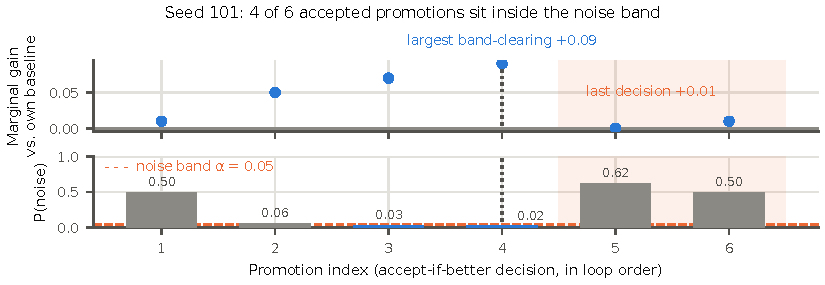
\includegraphics[width=0.96\linewidth]{../figures/exp4_stopping_seed101.pdf}
  % source figure (generated by `mdi report`, do not edit):
  %   exp4_stopping_seed101.pdf <- data/derived/exp4/promotions.json
  %   (rows + stopping[] for seed 101, alpha=0.05)
  \caption{Regimes seed 101: held-out gain per accepted decision against its
    noise probability. Four of the six do not clear the $\alpha{=}0.05$ band;
    the largest that clears is \#4 ($+0.09$), and the two taken after it
    measure $+0.00$ and $+0.01$.}
  \label{fig:loop-remeasure}
\end{figure}
